\section{Instalasi}
Instalasi pada kali ini menggunakan 2 sistem operasi yaitu Windows 10 x64 dan Ubuntu 19.04. Hal yang dibutuhkan adalah laptop dengan os windows atau ubuntu dan internet.
\subsection{Instalasi Anaconda 3 Windows 10 x64}
Hal yang harus diperhatikan sebelum melakukan instalasi \textit{Anaconda Python}
\begin{enumerate}
 \item \textit{Download Anaconda Python} https://www.anaconda.com/distribution/
 \item Perhatikan versi dari sistem operasi yang digunakan (versi 32bit atau 64bit)
 \item Download file anaconda yang sesuai dengan versi sistem operasi (32bit atau 64bit)
\end{enumerate}

Berikut langkah-langkah instalasi anaconda.
\begin{enumerate}
\item Buka aplikasi \textit{installer Anaconda} yang telah didwonload lalu akan muncul  gambar \ref{langkah1}, lalu pilih run untuk menjalankan proses instalasi. 
\begin{figure}[H]
        \centerline{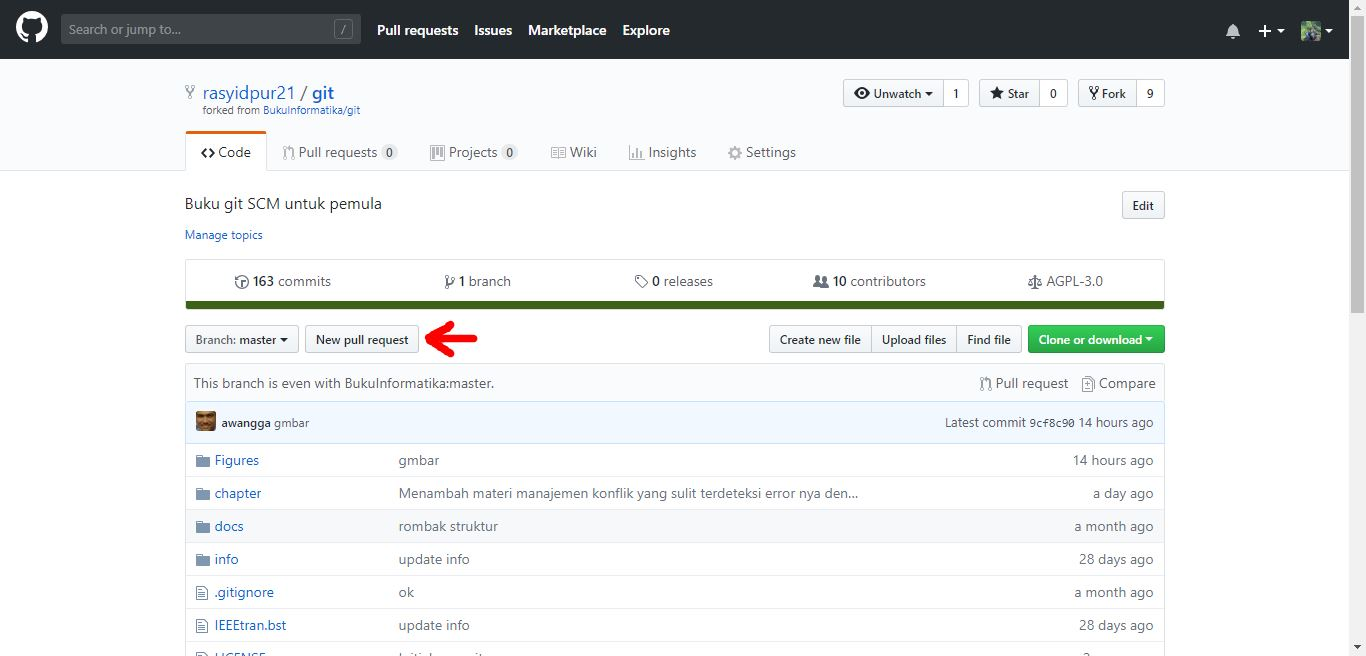
\includegraphics[scale=0.75]{figures/1}}
        \caption{Run Setup Anaconda}
		\label{langkah1}
\end{figure}

\item Tunggu hingga \textit{setup loading} selesai seperti pada gambar \ref{langkah2}.
\begin{figure}[H]
        \centerline{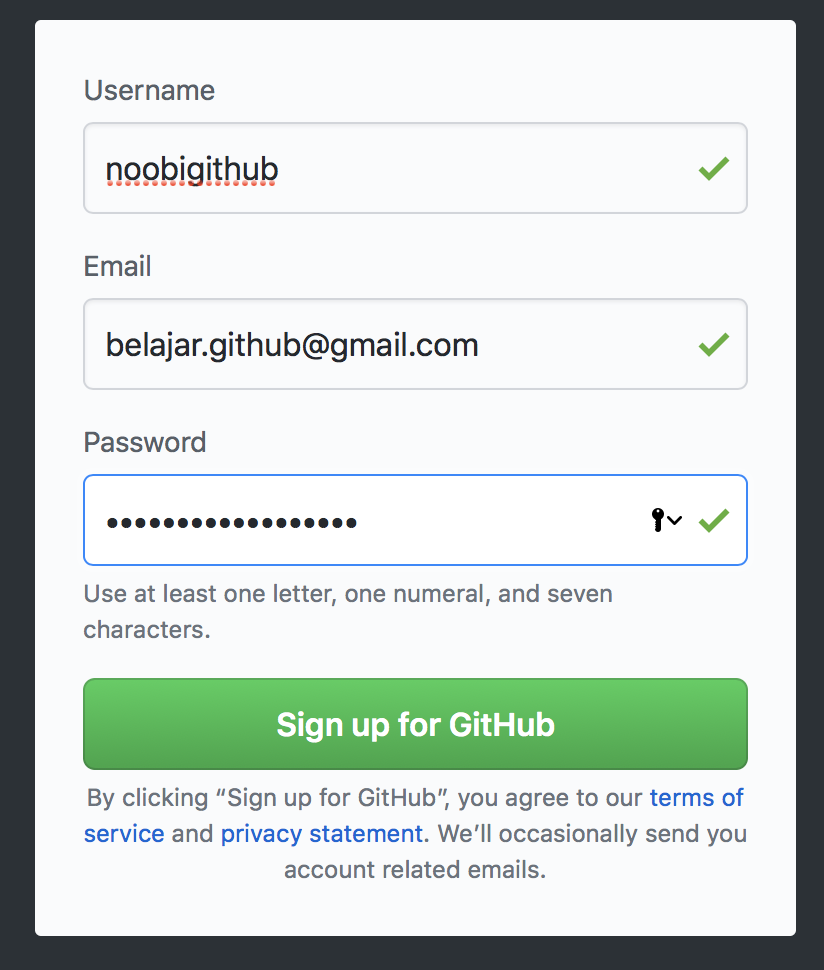
\includegraphics[scale=0.75]{figures/2}}
        \caption{Setup Loading}
		\label{langkah2}
\end{figure}

\item Jika \textit{setup loading} telah selesai, maka klik \textit{next} seperti pada gambar \ref{langkah3}.
\begin{figure}[H]
        \centerline{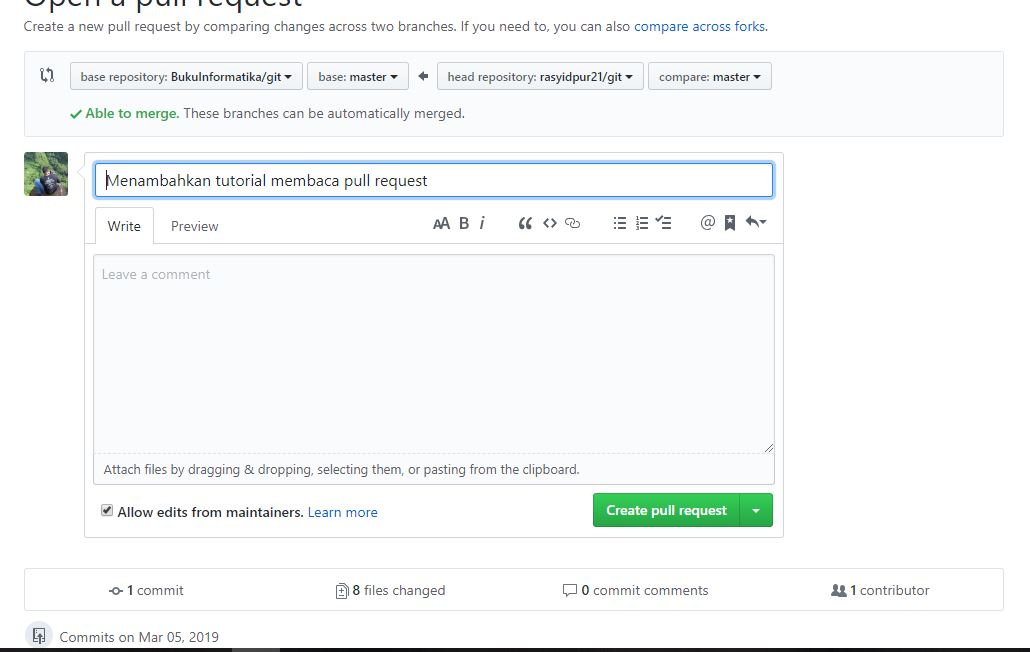
\includegraphics[scale=0.75]{figures/3}}
        \caption{Welcome to Anaconda Setup}
		\label{langkah3}
\end{figure}

\item Pada \textit{License Agreement} klik \textit{I Agree} karena jika teman-teman tidak menyetujui lisensi anaconda maka teman-teman tidak akan bisa melanjutkan proses instalasi. lakukan langkah ini seperti pada gambar \ref{Figureanaconda3}

\begin{figure}[H]
    \centering
    
\includegraphics[scale=0.75]{figures/4}
    \caption{\textit{License Agreement}}
    \label{Figureanaconda3}
\end{figure}


\item Kemudian pilih \textit{Just Me(Recomended)} agar sesuai dengan komputer yang digunakan, kemudian klik \textit{next} seperti pada gambar \ref{Figureanaconda4}.

\begin{figure}[H]
    \centerline{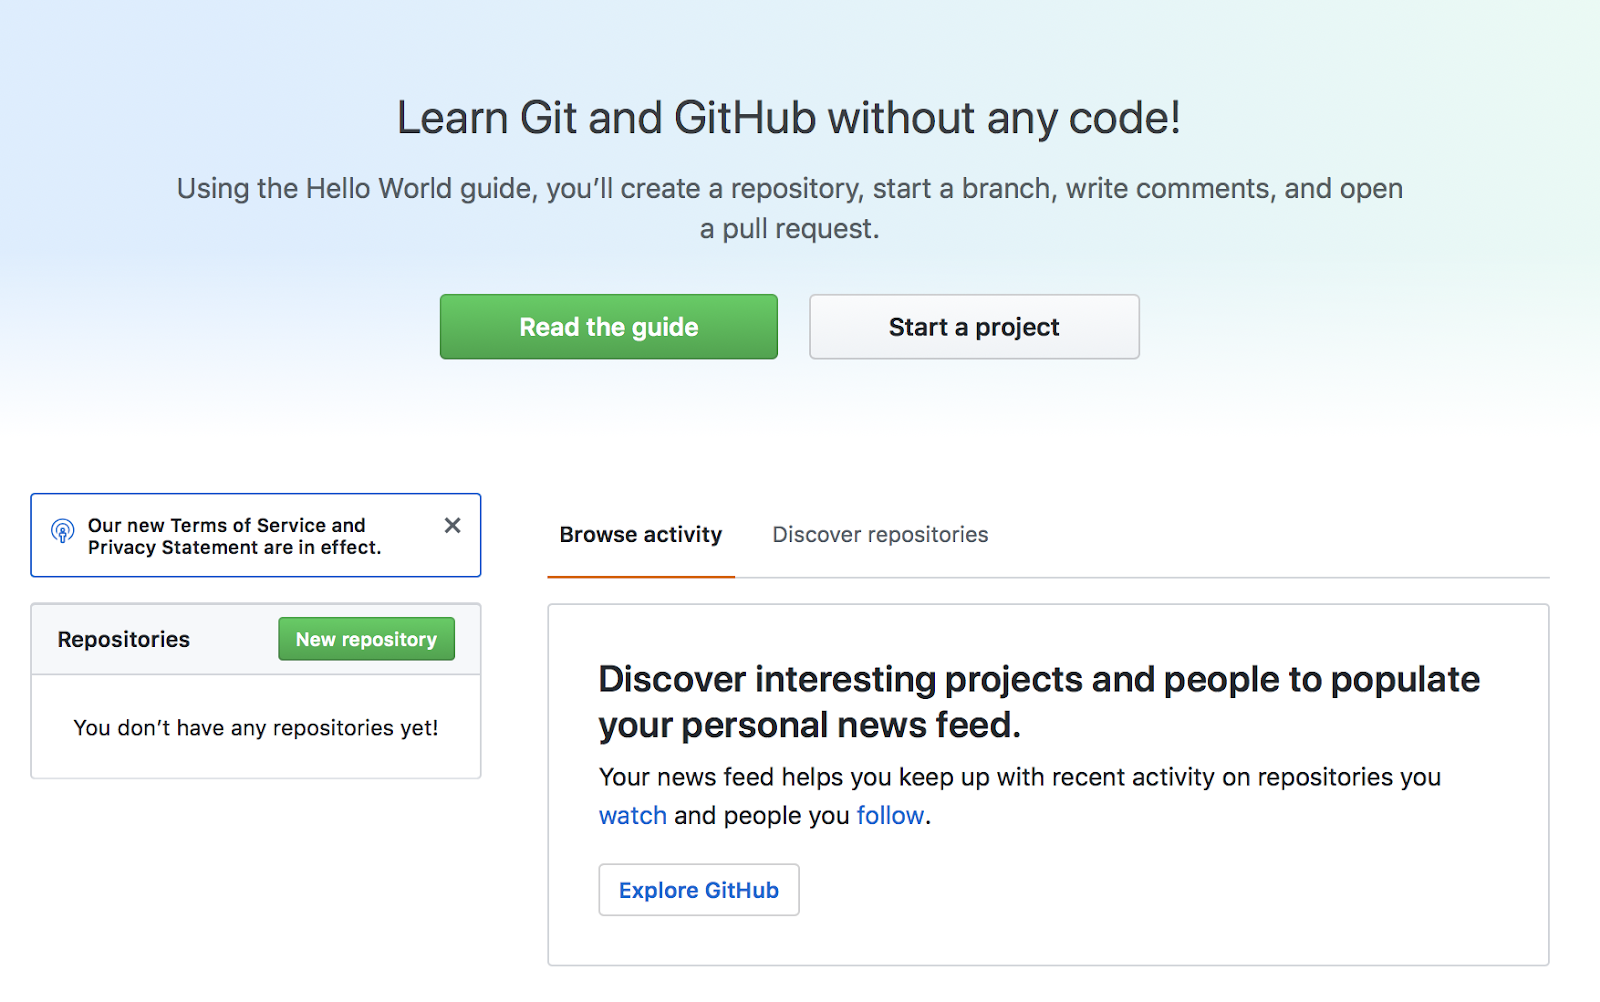
\includegraphics[scale=0.75]{figures/5}}
    \caption{\textit{Just Me(recomended)}}
    \label{Figureanaconda4}
\end{figure}


\item Kemudian pilih directori tempat kita akan \textit{menginstall anaconda} seperti pada gambar \ref{Figureanaconda5}

\begin{figure}[H]
    \centering
    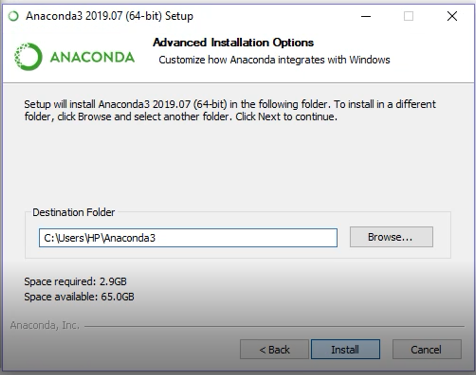
\includegraphics[scale=0.75]{figures/6}
    \caption{\textit{Pilih lokasi}}
    \label{Figureanaconda5}
\end{figure}

\item Kemudian centang \textit{Add Anaconda to my Path environtment variable}, agar saat melakukan instalasi  \textit{package anaconda, package} tersebut akan langsung tertuju ke \textit{path anaconda} tidak ke aplikasi yang lain. kemudian Klik \textit{install} seperti pada gambar \ref{Figureanaconda6}.

\begin{figure}[H]
    \centering
    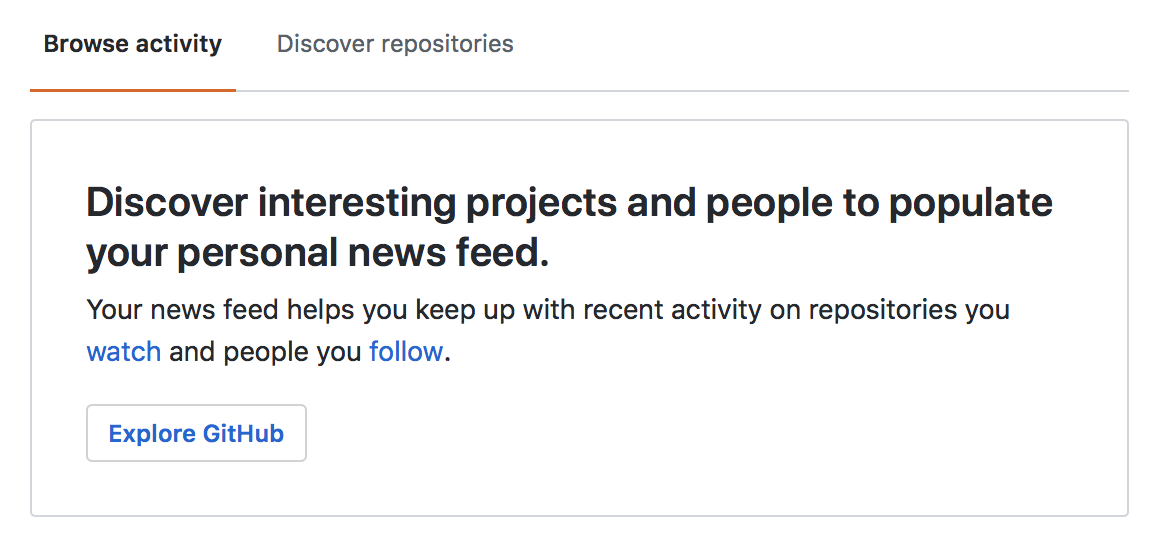
\includegraphics[scale=0.75]{figures/7}
    \caption{\textit{Centang Anaconda to my PATH}}
    \label{Figureanaconda6}
\end{figure}

\item Tunggu sampai proses \textit{installasi} selesai seperti pada gambar \ref{Figureanaconda7}.

\begin{figure}[H]
    \centering
    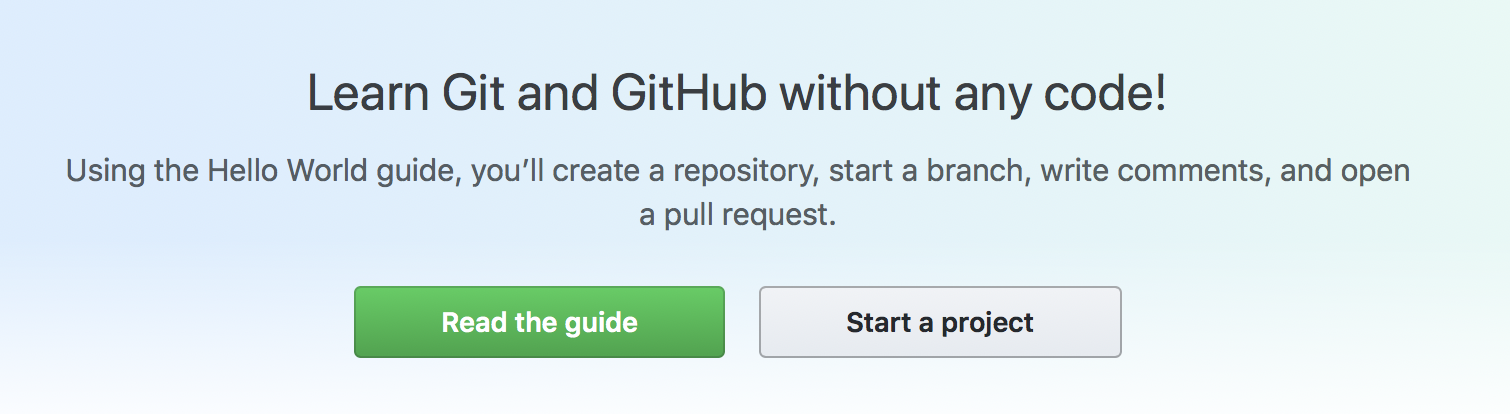
\includegraphics[scale=0.75]{figures/8}
    \caption{\textit{Waiting Installation Complete}}
    \label{Figureanaconda7}
\end{figure}

\item Apabila instalasi telah selesai  maka akan terlihat seperti gambar \ref{Figureanaconda8}, kemudian klik \textit{next}
\begin{figure}[H]
    \centering
    
\includegraphics[scale=0.75]{figures/9}
    \caption{\textit{Installation Complete}}
    \label{Figureanaconda8}
\end{figure}

\item apabila muncul gambar \ref{Figureanaconda70}, maka klik \textit{next}
\begin{figure}[H]
    \centering
    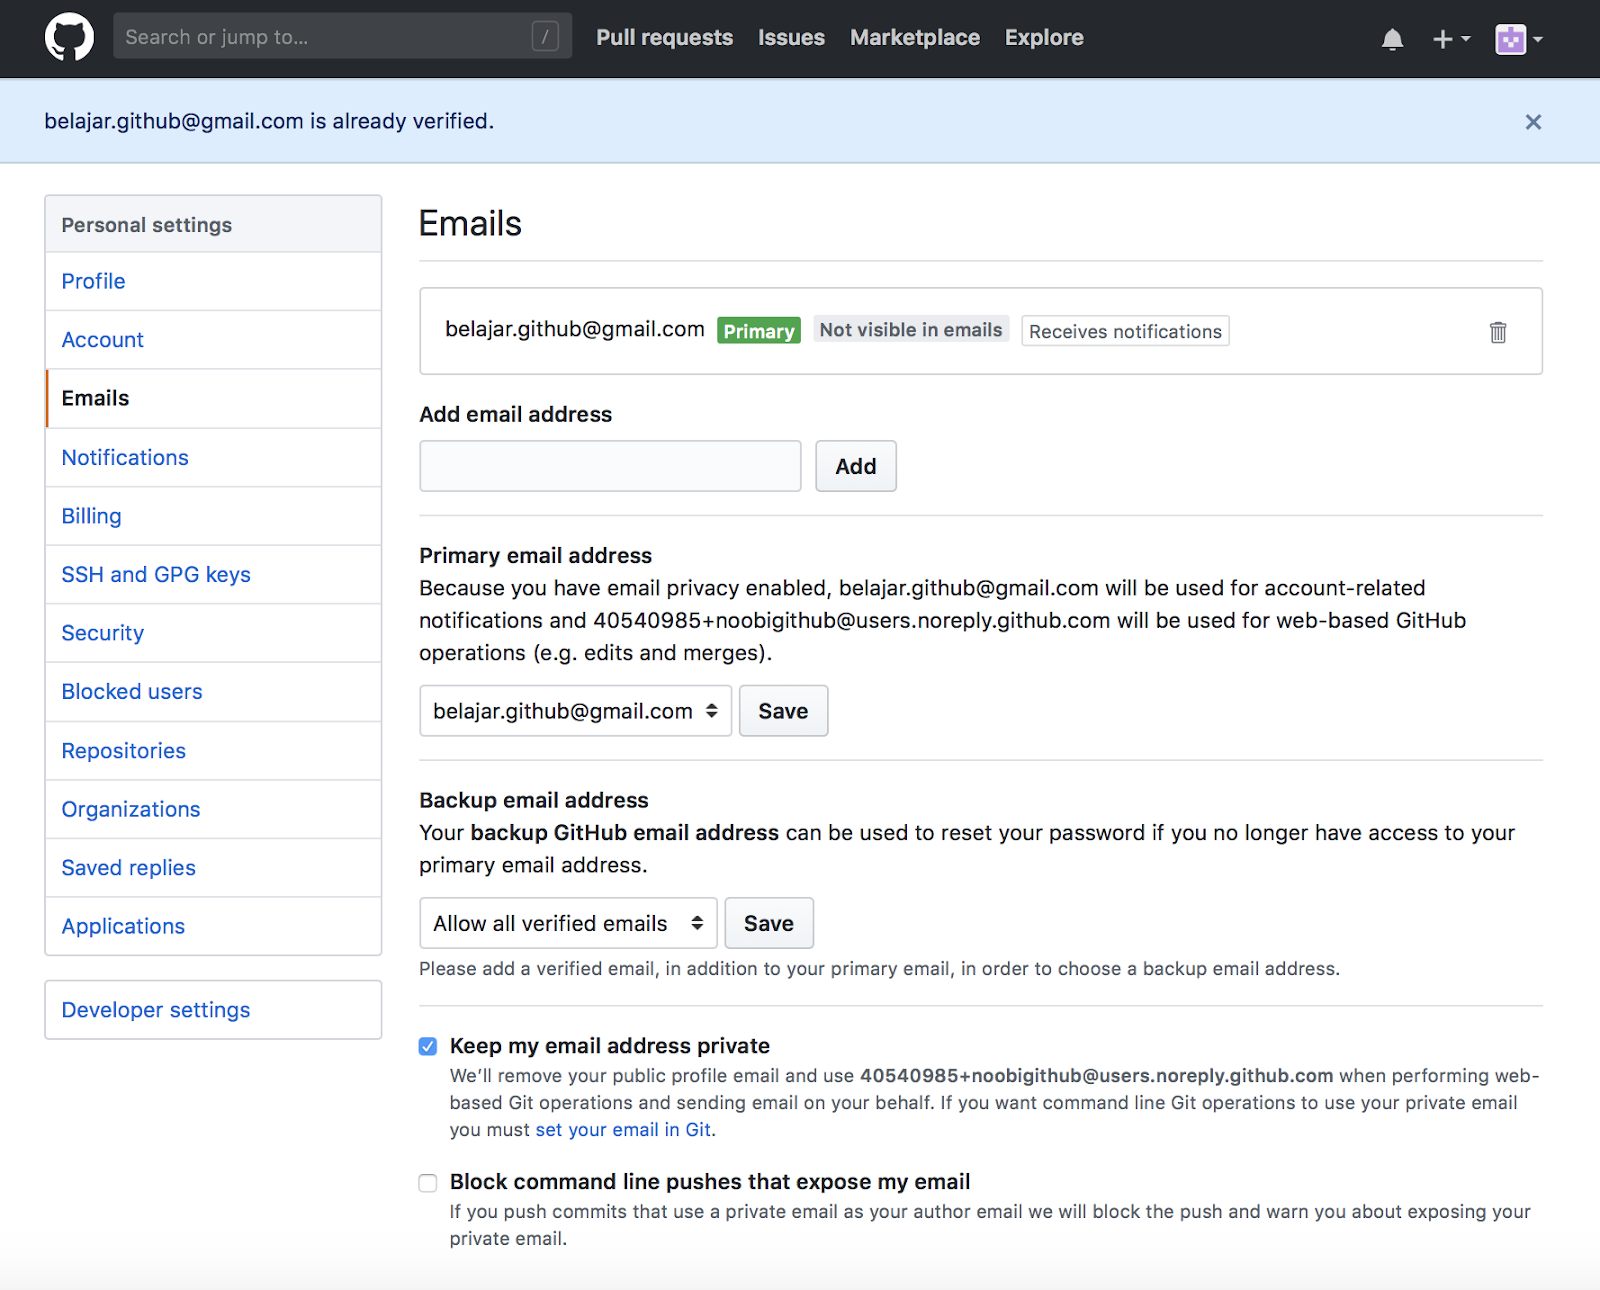
\includegraphics[scale=0.75]{figures/10}
    \caption{\textit{Anaconda+JetBrains}}
    \label{Figureanaconda70}
\end{figure}

\item Jika instalasi telah selesai maka akan ada ucapan terima kasih telah menginstall anaconda 3 seperti pada gambar \ref{Figureanaconda9}, hal ini menandakan bahwa teman-teman telah selesai dan berhasil melakukan instalasi anaconda. Kemudian klik \textit{finish} untuk mengakhiri instalasi.

\begin{figure}[H]
    \centering
    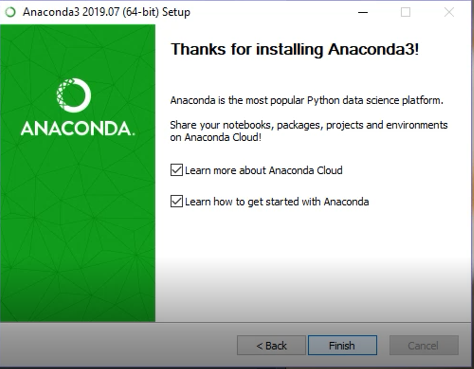
\includegraphics[scale=0.75]{figures/11}
    \caption{\textit{Thanks for install Anaconda}}
    \label{Figureanaconda9}
\end{figure}
\end{enumerate}

\subsection{Update Anaconda dan Spyder}
Kenapa kita harus melakukan update anaconda dan spyder? melakukan update diperlukan agar software yang kita gunakan merupakan software yang terbaru, karena versi lama dan versi baru akan memiliki banyak perbedaan dan akan menjadi masalah nantinya ketika kita membuat program atau mengimportkan modul-modul python yang digunakan.
Berikut cara mengupdate Spyder:
\begin{enumerate}
\item Buka anaconda prompt, lalu ketikkan perintah conda update spyder
\item Konfirmasi update dengan mengetikkan y, lalu tekan enter
\item Tunggu hingga installan selesai
\end{enumerate}
Berikut cara mengupdate Anaconda:
\begin{enumerate}
\item Buka anaconda prompt, lalu ketikkan perintah conda update anaconda
\item Konfirmasi update anaconda dengan mengetikkan y dan kemudian tekan enter
\item Tunggu hingga installan selesai
\end{enumerate}

\subsection{Instalasi Anaconda Ubuntu 19.04}
Untuk instalasi python pada Ubuntu 19.04 dibutuhkan sebagai berikut:

\begin{enumerate}
\item Internet
\item Anaconda installer (64bit or 32bit)
\item enter, dan yes atau no
\end{enumerate}

Ikuti langkah berikut:
\begin{enumerate}
\item Pertama kita kunjungi situs \textbf{\textit{https://www.anaconda.com/distribution/\#download-section}} seperti gambar ~\ref{anacondadownload} dan pilih \textbf{64-Bit (x86) Installer (517 MB)}
\begin{figure}[H]
\centering
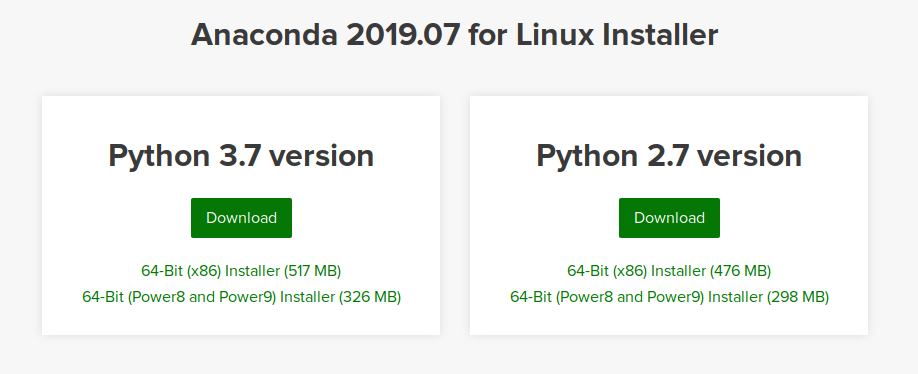
\includegraphics[width=1\textwidth]{figures/ubuntu/anacondadownload.png}
\caption{Gambar halaman download}
\label{anacondadownload}
\end{figure}

\item Kedua kita buka \textit{\textbf{terminal}} kita lalu arahkan ke direktori kita menyimpan file download anaconda

\item Ketiga kita ketikkan sebagai berikut \textbf{bash \textit{namafileanaconda}.sh} lalu enter, contoh seberti gambar \ref{anacondabash}
\begin{figure}[H]
\centering
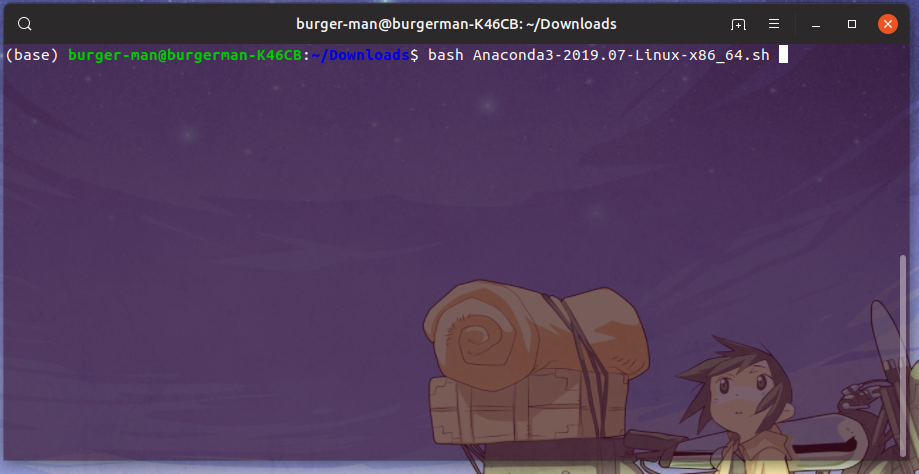
\includegraphics[width=1\textwidth]{figures/ubuntu/anacondabash.png}
\caption{Gambar install anaconda}
\label{anacondabash}
\end{figure}

\item Setelah itu, tekan \textbf{ENTER} saja seperti gambar \ref{anacondaenter}
\begin{figure}[H]
\centering
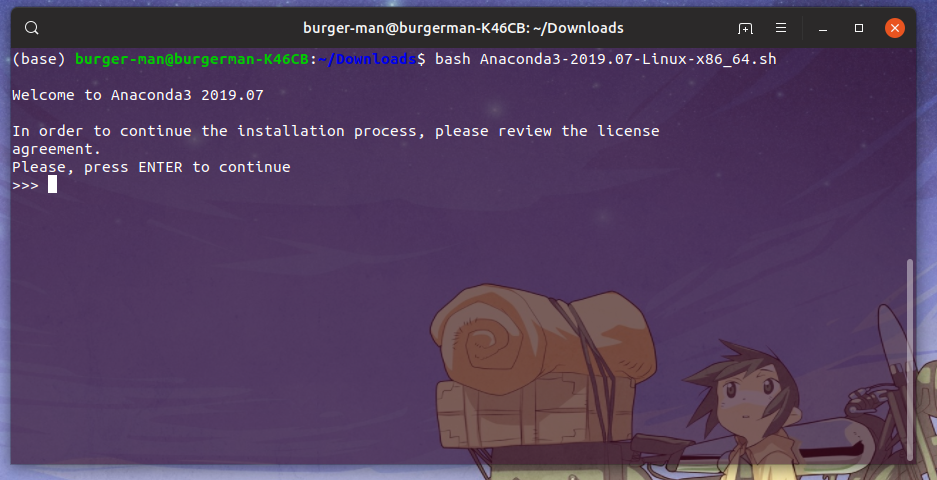
\includegraphics[width=1\textwidth]{figures/ubuntu/anacondaenter.png}
\caption{Gambar eksekusi anaconda}
\label{anacondaenter}
\end{figure}

\item Lalu akan muncul sebuah tulisan \textbf{End User License Agreement} seperti gambar \ref{entertrus}, tekan \textbf{ENTER} dan tahan hingga seperti gambar 
\begin{figure}[H]
\centering
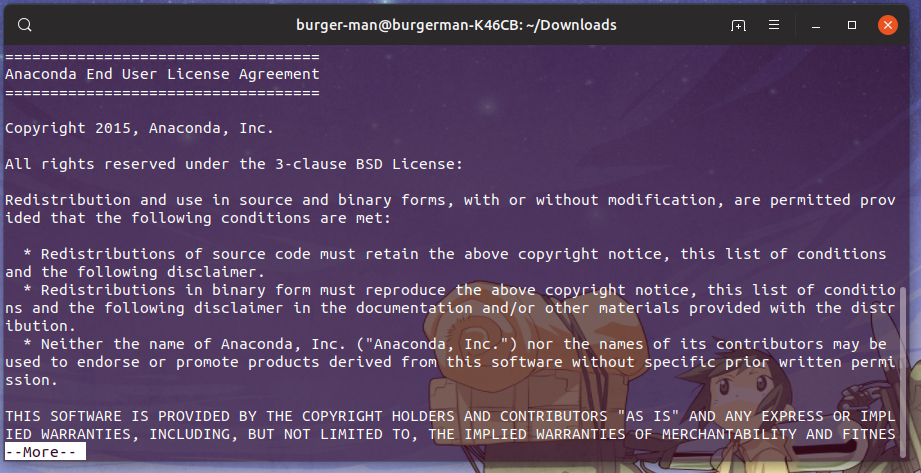
\includegraphics[width=1\textwidth]{figures/ubuntu/entertrus.png}
\caption{Gambar anaconda license agreement}
\label{entertrus}
\end{figure}
\begin{figure}[H]
\centering
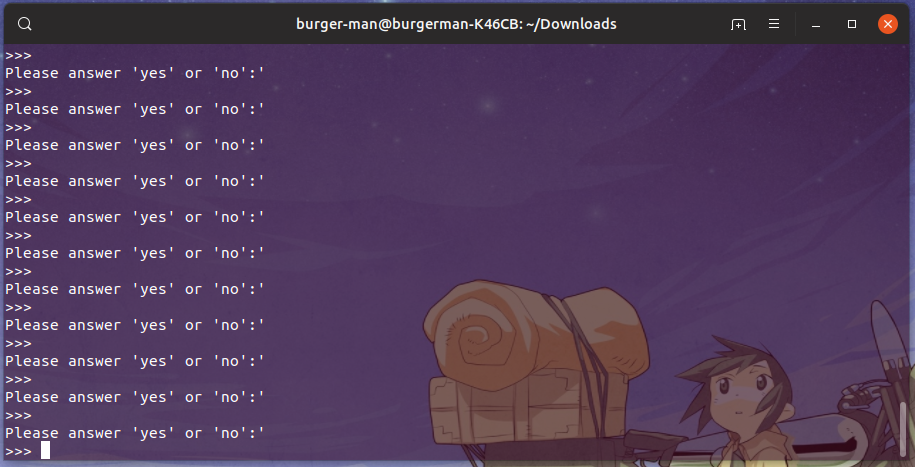
\includegraphics[width=1\textwidth]{figures/ubuntu/enterkekgini.png}
\caption{Gambar perintah yes or no}
\label{enterkekgini}
\end{figure}

\item Lalu setelah muncur perintah \textbf{\textit{'yes' or 'no'}} ketik \textbf{\textit{yes}} lalu enter

\item Setelah itu muncul path direktori instalasi anaconda kita seperti gambar \ref{enterpath} lalu tekan enter
\begin{figure}[H]
\centering
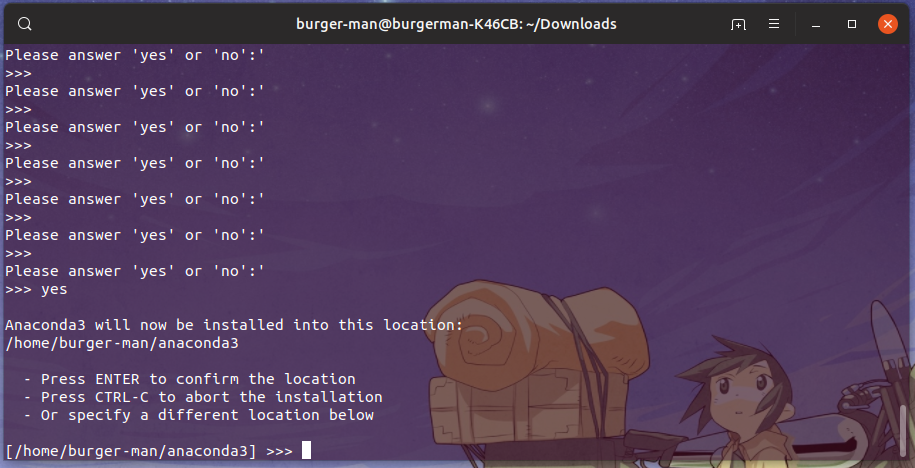
\includegraphics[width=1\textwidth]{figures/ubuntu/enterpath.png}
\caption{Gambar path anaconda}
\label{enterpath}
\end{figure}

Setelah kita selesai instalasi anaconda jangan lupa juga untuk menginstal spyder ide, caranya seperti berikut:
\begin{enumerate}

\item ketikkan perintah \textbf{\textit{sudo apt install spyder3 -y}} seperti gambar \ref{installspyder3}
\begin{figure}[H]
\centering
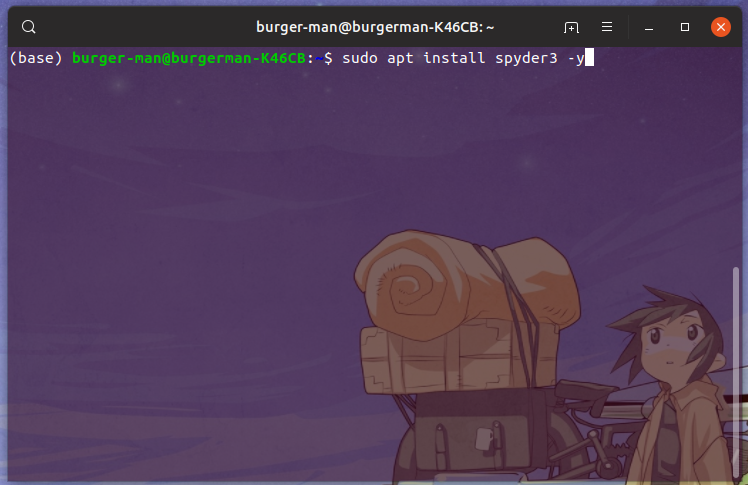
\includegraphics[width=1\textwidth]{figures/ubuntu/installspyder3.png}
\caption{Gambar perintah install spyder3}
\label{installspyder3}
\end{figure}

\item lalu jalankan dengan perintah \textbf{\textit{spyder}} atau \textbf{\textit{spyder3}}
\end{enumerate}

\end{enumerate}

\subsection{Konfigurasi \textbf{\textit{Python}}}
Setelah kita selesai instal Anaconda dan Spyder, selanjutnya kita akan mempelajari bagaimana cara setting environments python kita? caranya sebagai berikut

\begin{enumerate}

\item pertama kita buka terminal kita lalu ketikkan perintah \textbf{export PYTHONPATH=\$PYTHONPATH:\textit{pathinstallasipythonkalian}} contoh seperti gambar \ref{setpath}, lalu enter
\begin{figure}[H]
\centering
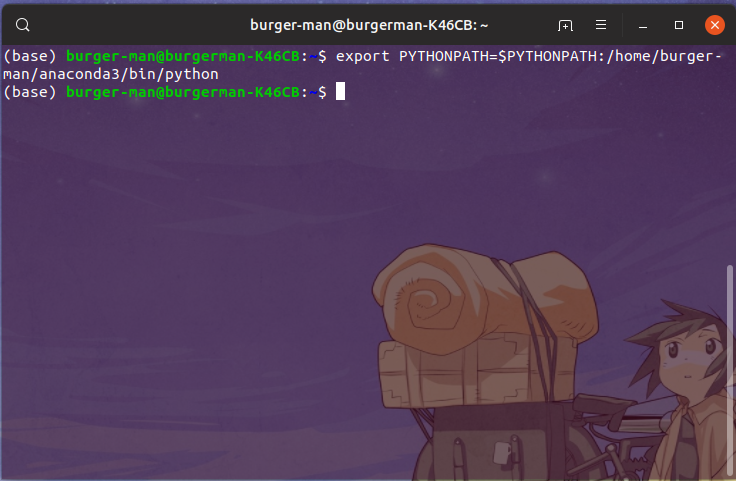
\includegraphics[width=1\textwidth]{figures/ubuntu/setpath.png}
\caption{Gambar setpath}
\label{setpath}
\end{figure}

\end{enumerate}

\subsection{Quiz 2}
\begin{enumerate}
\item Sistem operasi apa yang digunakan untuk instalasi pada buku ini?\\
a) Ubuntu dan Windows\\
b) Usus buntu dan Jendela\\
c) Penguin dan Kaca\\
d) Hewan dan Benda

\item Apa yang harus diperhatikan ketika ingin download Anaconda?\\
a) Kamu\\
b) Dia\\
c) Aku\\
d) Versi Sistem Operasi

\item Ubuntu versi berapa pada instalasi buku ini??\\
a) 19.04\\
b) 19.10\\
c) 19.99\\
d) 19.90

\item Apakah berbeda instalasi Anaconda pada windows dan linux?
a) Ya\\
b) Tidak

\item Apa yang kita memerlukan internet untuk instal Anaconda?\\
a) Ya\\
b) Tidak
\end{enumerate}